% Copyright (C) 2019 Cui Jialiang ( SESS, PKU ). All rights reserved.

\chapter{基于CNN和RNN的像素级别跟踪算法}
本章是本文的重点,将详细介绍本研究的理论创新.
\par
本研究所作的重点工作实际上是运用了深度学习技术,结合加密-解码结构的图像分割算法,加入RNN等结构实现了像素级别目标跟踪.具体算法结构,实现细节,训练等将在本章重点介绍.本章后文中将称本研究中提出的基于CNN和RNN的像素级别跟踪算法为本算法.

\section{算法简介}
本算法将首先基于用于实现静态图像分割的U-Net\supercite{ronneberger2015u}的多级降级-升级卷机神经网络结构.和处理静态图片的图像分割算法不同,我们将在这个多级网络结构中加入Conv-LSTM结构.
\par
与纽约大学2017年实现的Conv-LSTM结构的跟踪算法不同的是,本文所采用的多级神经网络将把Conv-LSTM加入各个卷机层级;而与U-Net,SegNet等多级分割算法不同的是,本文将在整个结构中多处穿插LSTM以得到一个时间连续的结果.

\subsubsection{算法的输入与输出}
同大多数跟踪算法类似,本算法的输入是一张张图片组成的视频序列,输出是像素级的跟踪结果.处理过程中需要始终存储并更新跟踪状态.
\par
具体的,在输入阶段,RGB传感器得到的图像由三张原图大小的灰度图像组成.不同于SIFT\supercite{lowe1999object},SURF\supercite{bay2006surf}等一些视觉图像处理算法,得益于深度学习方法在张量理解的优势,本算法将直接接受多波段的彩色图片为输入,这样能获得更大的输入空间.
\par
事实上,由于该输入需要被送入深度神经网络,为了更好的得到归一化的训练结果,本算法在输入阶段需要对输入数据进行归一化至$[0,1]$.对于三个波段都在$[0,255]$取值范围内的一个简单的归一化方法是:
\par
\begin{equation}\label{equ:input_norm}  input_{normlized} = \frac{input_{origin}}{255}  \end{equation}
\par

\subsubsection{算法的处理时效性}
% TODO 实时处理图(ppt)
本算法实际上是一个可以实时执行的跟踪算法.对于一个待提取跟踪目标的视频,本算法产生结果并不需要读入整个视频,只需输入当前与之前时刻的帧即可.即在跟踪过程中,每读入一张图片即进行一次处理.这使得在拥有一定量的计算资源时,本算法可以进行实时处理,即接收的图像结果的同时给出跟踪结果/
\par
对于$n$帧的视频,本算法的时间复杂度是$O(n)$,即增加视频长度只会线性增加算法处理所需的时间.

\section{基于CNN和RNN的像素级别跟踪模型在空间维度的处理}
\par
\begin{figure}[htbp!]
    \centering
    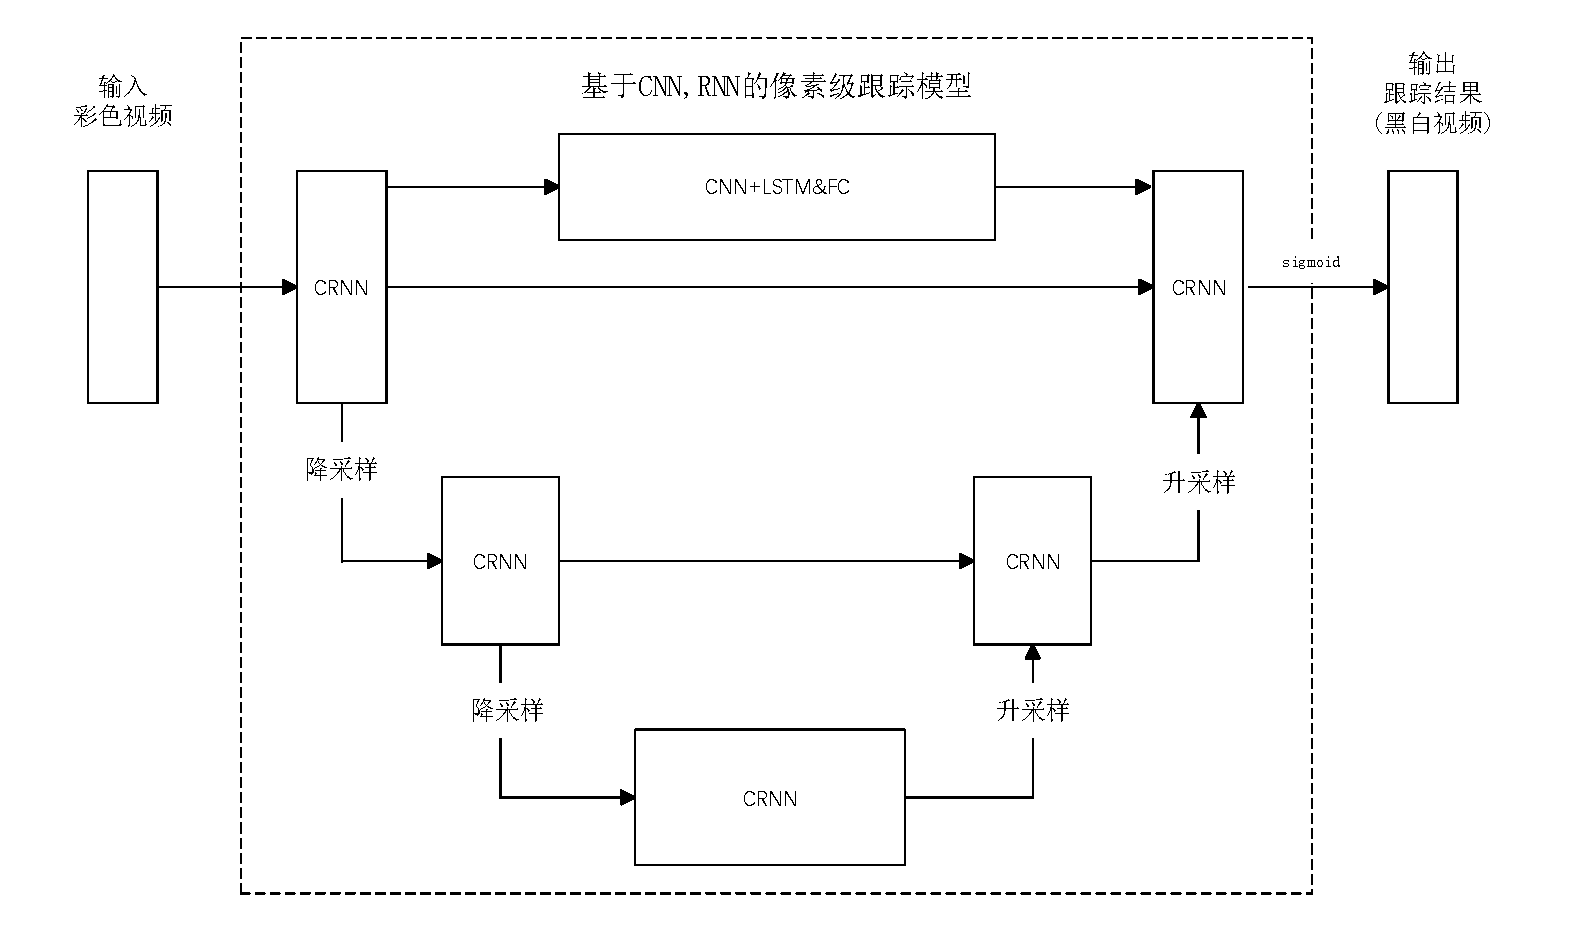
\includegraphics[width = 1.\textwidth]{chap/img/space_process.pdf}
    \caption{本算法在空间维度对单张图片的处理(这里略去了处理时间维度的RNN)}
    \label{fig:space_process}
\end{figure}
\par
类似与U-Net的结构,本文的卷机网络部分也将有多个降级和升级结构;每个降级结构包括几个卷积层,使用池化结构进行降级;每个升级部分采用升卷积进行升级处理.在降级过程中,图片数据的尺寸大小会衰减,同时等比例增加其波段范围.对于3层的结构,最小级的波段将有128个.这个多级结构的设计理念是为了处理多尺度问题;浅层的级别能很好的处理细节问题,但对宏观的把控会较弱,具体表现为可能会出现噪声点;深层的结构对宏观把控好,但对边界处理较弱.升级结构能将浅层处理得到的边界信息与深层处理得到的宏观信息相结合,得到一个更好的结果.

\par
\begin{figure}[htbp!]
    \centering
    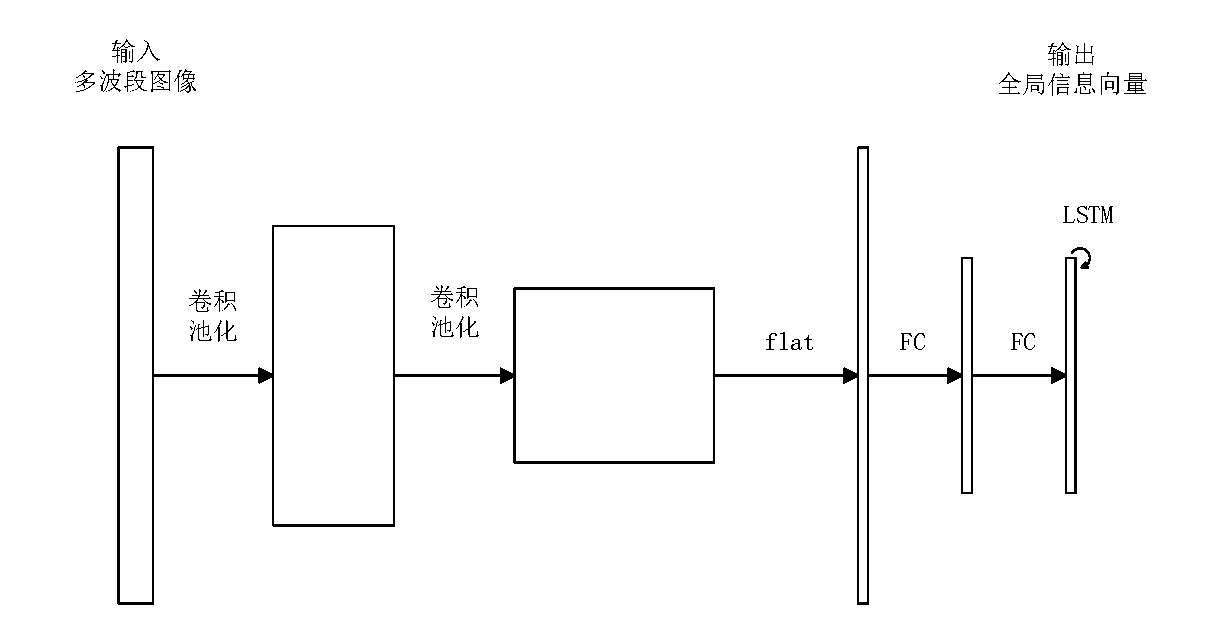
\includegraphics[width = 1.\textwidth]{chap/img/CNN_FCLSTM.pdf}
    \caption{cnn fc lstm}
    \label{fig:CNN_FCLSTM}
\end{figure}
\par
\subsection{多尺度思想的引入}

\section{基于CNN和RNN的像素级别跟踪模型在时间维度的处理}
\par
\begin{figure}[htbp!]
    \centering
    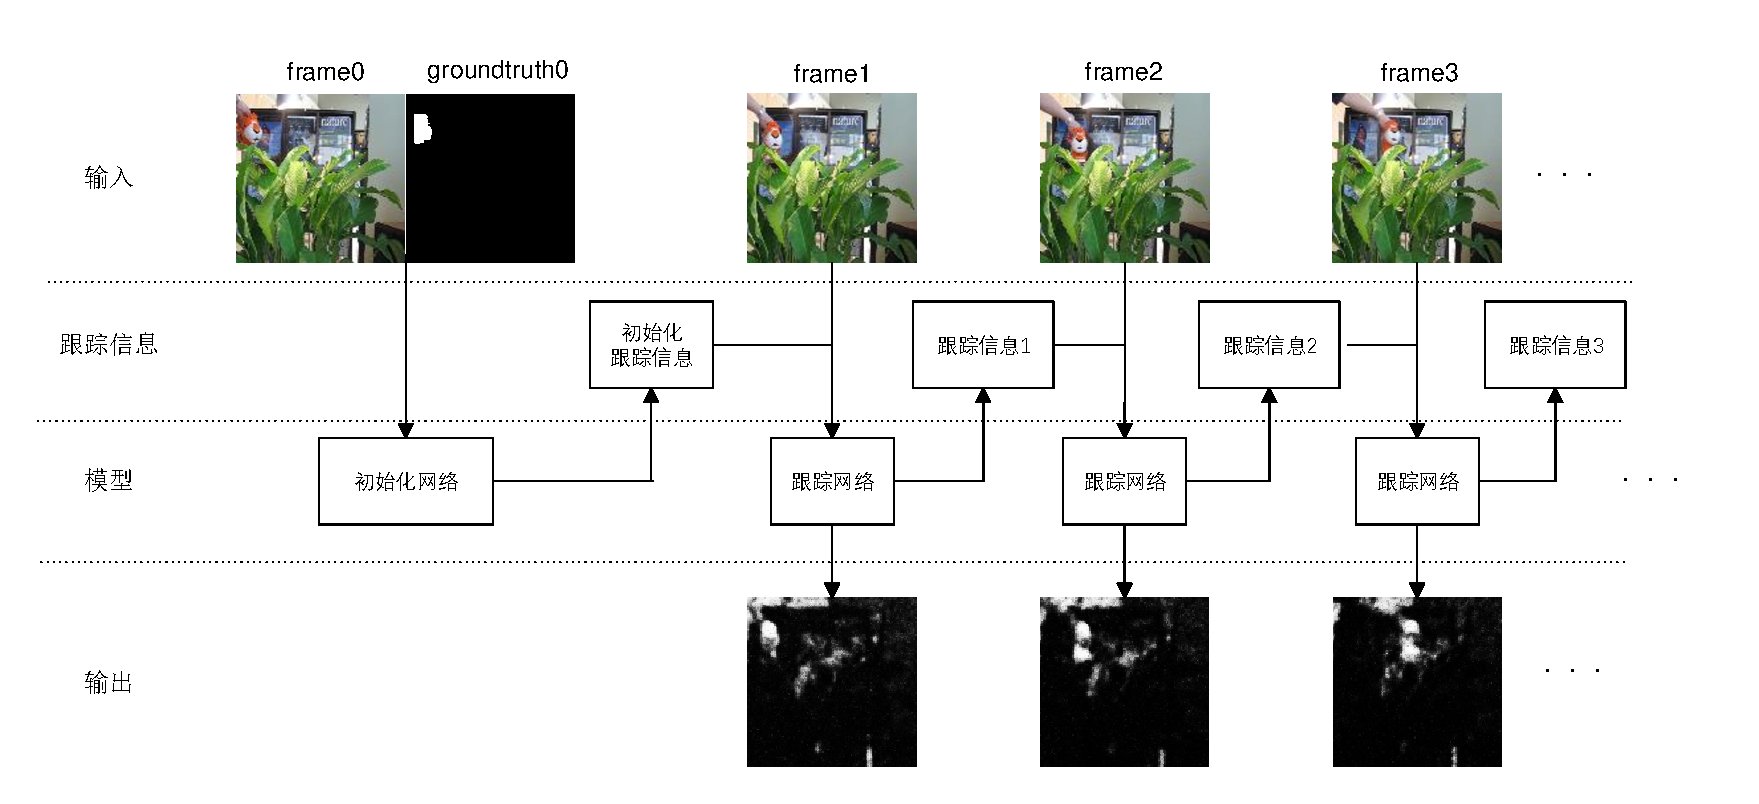
\includegraphics[width = 1.\textwidth]{chap/img/time_process.pdf}
    \caption{本算法在时间维度的大致处理思路}
    \label{fig:time_process}
\end{figure}
\par
在时间尺度,本研究的算法将主要采用LSTM算法解决问题.具体的,LSTM单元将被加入到各个层级当中.LSTM在各种跟踪算法中有广泛应用,但大多数算法仅仅将其作为对最后结果的处理手段.本研究的算法将把LSTM作为所有的中间状态记录单元.
\subsection{跟踪状态}
\subsection{跟踪系统初始化}